\documentclass{article}
\usepackage{arxiv}
\usepackage[T1]{fontenc}
\usepackage[utf8]{inputenc}
\usepackage{amsmath,amssymb,amsthm}
\usepackage{booktabs,tabularx,array,longtable}
\usepackage[numbers,sort&compress]{natbib}
\usepackage{microtype}
\usepackage{xcolor}
\usepackage{graphicx}
\usepackage{pgfplots}
\pgfplotsset{compat=1.18}
\usepackage{url}
\usepackage[colorlinks=true,linkcolor=black,citecolor=black,urlcolor=blue!45!black]{hyperref}
\hypersetup{pdftitle={Technical Supplement: Description Logic Programs Revisited},pdfauthor={Raphael Volz}}
\renewcommand{\shorttitle}{Revisiting Description Logic Programs}
\renewcommand{\headeright}{Technical supplement}
\renewcommand{\undertitle}{Preprint manuscript}
\newtheorem{proposition}{Proposition}
\newcommand{\lfp}{\operatorname{lfp}}
\newcommand{\TOP}{\mathsf{TOP}}
\newcommand{\code}[1]{\texttt{#1}}
\newcolumntype{Y}{>{\raggedright\arraybackslash}X}
\title{Technical Supplement:\\Description Logic Programs Revisited}
\author{Raphael Volz\\Pforzheim University}
\date{9 September 2026}

\begin{document}
\maketitle
\begin{abstract}
This supplement provides the semantic corrections, preservation arguments,
experimental protocols, complete result tables, and reproducibility details
supporting \emph{Description Logic Programs Revisited: The Benefits and Limits
of Specialized Ontology Reasoning}. It retains the technical evidence behind
the main paper's claims, including adverse outcomes and limitations. Earlier
experiments and their data are preserved. The Bach comparison adds observations
of the thesis's original examples and retains a diagnosed external update
discrepancy.
\end{abstract}

\section{Original work, semantics, and reconstruction}
\subsection{What is inherited from the thesis}
The thesis provides the DLP-oriented problem decomposition, position-sensitive
constructor translation, instance and schema reasoning services, and maintenance
under changes to a knowledge base. Chapters 5--7 are the main implementation
reference; chapter 8 supplies taxonomy, restriction, and update workload designs.
The 2003 materialized-ontology paper already discusses changing both extensional
facts and intensional rules~\cite{volz2003maintenance}.

The reconstruction compiles RDF-encoded OWL expressions into immutable Horn
rules. RDFLib supplies RDF parsing; it does not establish the correctness of the
OWL-to-Horn translation. The engine uses relation indexes, semi-naive deltas,
explicit equality with congruence, integrity constraints, and a distinction
between assertions and derived facts. It supports a documented DLP fragment,
not full OWL DL, OWL Full, or complete OWL 2 profile conformance.

The local DLP L0--L3 names follow constructor-position distinctions in the
reconstruction. For example, an existential antecedent
$\exists R.C\sqsubseteq B$ is a Horn pattern match, whereas an existential
consequent $A\sqsubseteq\exists R.C$ requires the witness-generating DLP L3 mode.
General disjunctive heads, property chains, keys, arbitrary datatype restrictions,
and maximum cardinality above one are outside the implemented contract.
Automatic literal value identity covers only stated string, numeric, and Boolean
families. Unsupported logical constructs fail explicitly.

Negative answers require a complete consistent computation; failure to derive
a fact is not derivation of its negation. Different IRIs are not presumed to
denote different individuals. DLP L3 uses Skolem witnesses; unrestricted evaluation
can fail to terminate on recursive existential ontologies, while configured
resource limits return an incomplete result. Retractions involving equality reconstruction or existential
witnesses use rematerialization. The certificate argument below does not extend
to those cases.

\subsection{Focused corrections and their significance}
The audit uses the thesis's printed page numbers; the one-based PDF page is 16
higher. Table~\ref{tab:errata} gives representative corrections. The repository's
longer errata includes the countermodels, conditional benchmark-count
corrections, and independent executable checks. These are findings from this
implementation review; they do not establish how the historical software behaved.

\begin{table}[ht]
\caption{Representative audited issues in the original thesis~\cite{volz2004}.
The corrections concern the printed specification; historical software behavior
cannot be inferred without its implementation and raw data.}
\label{tab:errata}
\small
\begin{tabularx}{\linewidth}{@{}p{0.17\linewidth}YY@{}}
\toprule
Location & Issue & Required interpretation or replacement \\
\midrule
Table 5.3, p.~122 & Subproperty and transitivity implications point in the wrong direction. & $P(x,y)\!\to\!Q(x,y)$ for $P\sqsubseteq Q$; $P(x,z)\land P(z,y)\!\to\!P(x,y)$ for transitivity. \\
\S5.4.4.2, p.~136 & Joint class-equivalence probes can interfere through equality. & Run the two subsumption probes in separate fresh states. \\
Eq.~(5.13), p.~140 & Exact inverse equality is inherited to a strict subproperty. & Inherit inverse inclusion, or require property equivalence for exact inverse equality. \\
Algorithm 6.1, p.~163 & A removed rule can retain an obsolete rederivation contribution. & Identify losses using old rules; restore only with current rules. \\
\S5.4.2.2, p.~133 & A stated distribution is false; explicit DNF need not be linear. & Correct the identity and retain factored structure or auxiliary predicates. \\
Tables 8.9--8.10 & Restriction columns and some population labels conflict with the generator description. & Validate generated counts; do not relabel unavailable historical measurements as reconstructed data. \\
\bottomrule
\end{tabularx}
\end{table}

Two examples show why the procedural findings matter. If
$C\sqsubseteq\{o\}$ and $D\sqsubseteq\{o\}$, a joint probe asserting $C(a)$ and
$D(b)$ identifies $a=o=b$ and obtains both cross-memberships. Yet $C=\{o\}$,
$D=\varnothing$ is a countermodel to $C\equiv D$. Fresh names alone do not
isolate tests under equality. For deletion, let $A(a)$ be explicit and let
$P(x)\leftarrow A(x)$ and $P(x)\leftarrow B(x)$ be the rules, with $B$ empty.
Removing the first rule must remove $P(a)$. An obsolete rederivation rewrite
can incorrectly preserve it.

These findings invalidate particular printed formulas or procedures, not the
entire research programme. The model-theoretic connection between the supported
languages and the usefulness of rule-based ontology evaluation do not depend
on the faulty examples. Conversely, successful modern tests cannot certify the
historical implementation or recover which datasets produced ambiguous old
timing entries. The audit also corrects its own earlier interpretation: loose
restriction scope in Example 5.4.2 is reported as ambiguous parentheses rather
than a separately proven semantic error. OWL's original direct semantics
provides an independent reference for the relevant constructors~\cite{owl2004}.

\section{Delta-sensitive unary evaluation}
For a recognized rule body $P_1(x),\ldots,P_k(x)$, let $I_i$ be its current
relation and $D_i$ the frontier for that relation. Duplicate predicates are
removed. The engine ingests the frontier before evaluation, so $D_i\subseteq I_i$.
The coalesced semi-naive result is
\begin{equation}
 J=\left(\bigcap_{i=1}^{k}I_i\right)\cap
   \left(\bigcup_{i=1}^{k}D_i\right).
 \label{eq:delta}
\end{equation}
The fixed plan first constructs the delta union and intersects the necessary
full relations. This can create a large temporary set even when a small full
relation already bounds every possible answer.

The selector rejects an empty required relation and handles an already bound
variable by exact membership tests. If a nonempty delta has the same cardinality
as its full relation, the subset invariant proves equality: every full-join
answer meets the delta condition. With a single nonempty delta, the engine uses
that set directly. Otherwise define $M=\sum_i|D_i|$, $s=\min_i|I_i|$, and let
$h\leq k$ count the nonempty deltas. The alternative branch is selected when
$M>ks$:
\begin{equation}
 T=\bigcap_i I_i, \qquad J=\bigcup_i(T\cap D_i).
 \label{eq:fullfirst}
\end{equation}
Set distributivity establishes equivalence with Eq.~\eqref{eq:delta}. Full
relations are considered in cardinality order, and delta filtering may stop
when its accumulated answer covers $T$. The selector uses current exact sizes;
it does not infer independence or estimate overlap from samples.

Under expected constant-time hashing, the full-first branch uses
$O(k\log k+ks+hs)$ work and $O(s)$ temporary tuple storage, excluding references
and emitted bindings. A simple scan accounting charges at most $ks$ for
copying/intersecting the full relations and $2hs$ for filtering and collecting
outputs. Since the branch is chosen only when $M>ks$,
\begin{equation}
 (k+2h)s\leq 3ks<3M.
\end{equation}
This is a scoped scan bound, not a three-competitive runtime theorem. Sorting,
allocation, hash collisions, Python dispatch, and unequal operation constants
are outside that inequality. Engine counters also omit work performed inside
C-level set operations.

An initial rule selected full-first at $M\geq s$. A pilot falsified it: 64
identical singleton deltas over 32-row full relations have a one-row union but
trigger many full intersections. The observed kernel slowdown was about
2.7-fold. The width-aware threshold was adopted before the final experiment,
and this adversary was added to its protocol. The pilot is development evidence;
the retained confirmatory samples concern the revised selector. Equality
reindexing and DRed variants preserve their applicable delta contracts; the
coalesced shortcut is not imposed on unrelated arbitrary delta relations.

\section{Bounded current-proof certificates}
\subsection{State and oracle}
Let $P,E$ be the old rules and explicit facts and let $D$ contain the old active
domain's generated $\TOP$ facts, including the private nonempty-domain
representative. Let $P',E',D'$ describe the complete proposed transaction state.
Write
\begin{equation}
 \mathcal M=\lfp(P,E\cup D),\qquad
 \mathcal M'=\lfp(P',E'\cup D').
\end{equation}
The incremental deletion setting is finite, positive, function-free, and
equality-free, with a complete old materialization. Denials are checked
separately. Existing explicit current facts already stop unnecessary deletion.

The oracle indexes only current rules of the form
$H(x)\leftarrow B_1(x),\ldots,B_m(x)$, with $m\geq1$ and exactly the same
variable in every atom. It excludes constants, binary atoms, multiple variables,
existential terms, and constraint heads. For subject $a$, the seed signature
contains predicates explicitly asserted of $a$ in $E'$, plus $\TOP$ precisely
when $a$ belongs to the current domain. Forward propositional Horn closure of
the signature gives a set of proved predicates.

Subjects with identical signatures share this computation. A cycle cannot
certify itself because old derived predicates are never seeds. Newly inserted
rules and assertions may supply valid replacement support: the oracle examines
the complete current candidate, not only the pre-transaction program. A positive
answer protects an old fact considered for deletion. Other oracle conclusions
are not inserted into the store. Ordinary evaluation must still create and
propagate new intermediate facts and consequences of newly inserted rules.

\subsection{Preservation argument}
\begin{proposition}[Sound current-proof protection]
Under the stated finite positive assumptions, DRed may additionally protect
queried old facts $C\subseteq\mathcal M'$ during overdeletion through the old
program, provided restoration evaluates current definitions of deleted
predicates, evaluates all inserted rules, and propagates new and restored facts
to a fixed point.
\end{proposition}
\begin{proof}
Every old fact has a finite derivation tree. When an old proof uses a removed
assertion, removed rule, or departed domain seed, deletion is seeded there and
propagates through that proof until it reaches a protected fact. A protected
fact has a finite current proof; substituting that proof makes the cut safe.
Current explicit and domain facts are safe leaves. Hence an unsupported old
fact cannot survive merely through cyclic old dependencies. Restoration uses
only current rules, so every restored consequence is sound.

For completeness, consider a finite current derivation. If all premises of a
rule survived but its old head was deleted, evaluating current definitions of
deleted predicates recovers that head. An inserted or restored premise triggers
ordinary delta propagation, and each inserted rule is evaluated. An unchanged
rule with all premises already in the complete old model cannot yield a
genuinely new head absent from that model. Induction over current derivation
height therefore recovers every current consequence.
\end{proof}

The unary oracle supplies the required subset by induction over its rule
firings. Every seed is current, and every added predicate follows from a
current rule and proved premises. Even an incomplete monotone exploration is
sound. This is a preservation argument for the implementation's interface,
not a machine-checked proof or a claim that the general principle is new.

\subsection{Budgets and expected failure modes}
The implementation allows at most 128 cached signatures and 100,000 dependency
visits per transaction. Exhaustion yields ``unknown'' and ordinary DRed
continues. These bounds restrict search, not total transaction time or memory:
index construction scans current rules and assertions, each query constructs or
retrieves a signature, and a context may contain many predicates. Search order
can change which contexts benefit, but never the soundness of a positive answer.

Shared signatures with independent surviving support should amortize the oracle
cost. Unsupported cycles provide no certificates and expose pure overhead.
Unique signatures stress the cache cap. Support that depends on binary rules
is intentionally outside the oracle, even when general DRed can recover it.
Thus a correct oracle can still be a poor default. Learning or hand-tuning a
dispatcher on these same cases would require a new held-out evaluation.

\section{Experimental protocol and validation}
The preserved baseline is commit
\code{b1254c441731ca4fdf32ea83570ff99aaa84ac2a}. Its original result file and
manifest are immutable. Commit \code{8ce254f} contains the preceding
modernization; commit \code{5531be4} records the research implementation and
evidence. The factorial experiment was run against a source snapshot whose
hashes and archive are preserved. Its four variants share access-path
specialization and differ only in fixed/adaptive unary planning and
ordinary/certificate-guided DRed. The fixed variant is not an archived checkout
of the historical baseline.

The final v3 protocol defines ten unary cases: five shapes at widths 8 and 64.
Each uses 2,048 subjects except the overlapping-singleton adversary with 32.
Eight support cases combine surviving alternate support, unsupported cycles,
mixed new support, and unique signatures with depth parameters 4 and 32 and
256 subjects. Depth $d$ generates predicates $C_0$ through $C_d$ plus an answer
predicate. Nine process blocks and four configurations yield 648 timed workers.
Seeded Latin-square rotations balance position over groups of four blocks;
the ninth is not fully balanced. No warm-up samples are discarded.

The primary endpoint is outer wall time of the complete \code{Engine.update},
including candidate validation, planning, indexing, deletion, and restoration.
Input generation, hashing, and outcome checks are outside that interval.
Per-case ratios are medians of the nine within-block ratios. Their paired
bootstrap intervals are descriptive; nine blocks on one host do not establish
population-wide significance. Earlier v1/v2 protocols and the failed pilot
are disclosed. The protocol was saved before the experiment, but was not
independently timestamped public preregistration.

Every worker checks its full result against fresh materialization and records
canonical input, rule, assertion, and actual closure hashes. Thirty-six small
controls additionally use an independently written finite-grounding evaluator.
The expected transaction digests in the primary artifact should not be confused
with direct inspection of internal assertion storage; randomized integration
tests separately compare that storage with independently maintained inputs.
Seventy-two separate processes measure additional Python allocations with
\code{tracemalloc}. Instrumented times never enter the timing summaries, and
these allocations exclude the pre-existing store and untraced native memory.

The host is an Apple M4 Max with 16 reported CPU cores, macOS 26.5.1 arm64,
Python 3.12.9, and RDFLib 7.6.0. Exclusive host use was not established: an
unrelated Bach report was rewritten during the primary timing window. Its
exact CPU overlap is unknown. All original samples are retained. A post-hoc
support replication used new seeds and 144 fresh workers, after the production
suite finished, to check the main conditional gain and adverse overhead.

The predeclared engineering screen required adaptive execution to have a
geometric mean update ratio at most one and no case above 10\% slowdown.
Certificates required consistent intended benefits and adverse overhead at most
10\%. Thresholds were not adjusted after the outcomes. The completed research
validation had 593 tests, including 1,458 exhaustive small relation/delta
combinations and 1,000 randomized mixed transaction states, plus independent
thesis-counterexample scripts, lint, and a package build. These validate the
stated implementation scope, not all OWL semantics.

\section{Results}
\subsection{Adaptive evaluation: work savings without an end-to-end gain}
\begin{table}[ht]
\caption{Complete-update unary results (nine paired process blocks). Milliseconds; ratio below one favors adaptive planning. Intervals are descriptive.}
\label{tab:unary}
\centering\small
\begin{tabular}{@{}lrrrrl@{}}
\toprule
Shape & Width & Fixed & Adaptive & Ratio & 95\% interval \\
\midrule
sparse-single & 8 & 10.623 & 10.628 & 1.0026 & [0.9768, 1.0123] \\
sparse-single & 64 & 100.506 & 99.957 & 1.0060 & [0.9624, 1.0209] \\
sparse-disjoint & 8 & 10.502 & 10.782 & 0.9961 & [0.9340, 1.0409] \\
sparse-disjoint & 64 & 103.556 & 103.567 & 0.9972 & [0.9734, 1.0473] \\
sparse-overlap & 8 & 0.271 & 0.269 & 1.0246 & [0.9672, 1.1895] \\
sparse-overlap & 64 & 2.132 & 2.147 & 1.0018 & [0.9945, 1.0201] \\
dense-overlap & 8 & 53.179 & 53.651 & 1.0019 & [0.9944, 1.0327] \\
dense-overlap & 64 & 688.126 & 697.530 & 1.0127 & [0.9814, 1.0303] \\
dense-selective & 8 & 42.324 & 41.733 & 0.9903 & [0.9777, 1.0194] \\
dense-selective & 64 & 656.392 & 667.461 & 0.9818 & [0.9378, 1.1023] \\
\bottomrule
\end{tabular}
\end{table}

The geometric mean of the ten paired ratios is 1.001446, with worst case
1.024637; every descriptive interval includes one. The candidate therefore
fails its at-most-one geometric-mean adoption requirement. This does not prove
that adaptation is generally harmful, but it supplies no basis for enabling
the feature by default.

At width 64 in the dense-selective case, delta-union input visits fall from
64,512 to zero, while 32 delta-filter visits produce the same 32 body matches.
Additional traced peak allocation falls only from 79,735,524 to 79,679,418
bytes. The complete transaction includes large assertion batches and index
updates, so a favorable kernel transformation need not change user-visible
latency. For sparse-single updates, the median fraction outside the internal
evaluator timer is 99.46\% at width 8 and 99.88\% at width 64. This diagnostic
suggests transaction preparation as a next target, but does not isolate its
individual causes or prove that all of that time can be removed.

\subsection{Certificates: conditional gains and adverse overhead}
\begin{table}[ht]
\caption{Certificate update ratios in the primary study and independent post-hoc replication. Each uses nine paired blocks per case.}
\label{tab:support}
\centering\small
\begin{tabular}{@{}lrrrl@{}}
\toprule
Shape & Depth & Primary & Replay & Replay 95\% interval \\
\midrule
alternate-support & 4 & 0.2977 & 0.3031 & [0.2992, 0.3085] \\
alternate-support & 32 & 0.1343 & 0.1323 & [0.1266, 0.1338] \\
unsupported-cycle & 4 & 1.1896 & 1.1784 & [1.1364, 1.1947] \\
unsupported-cycle & 32 & 1.1859 & 1.1879 & [1.1537, 1.2280] \\
mixed-new-support & 4 & 0.3730 & 0.3819 & [0.3658, 0.3948] \\
mixed-new-support & 32 & 0.1478 & 0.1495 & [0.1477, 0.1532] \\
unique-signatures & 4 & 0.9062 & 0.9053 & [0.9000, 0.9170] \\
unique-signatures & 32 & 0.7907 & 0.7849 & [0.7724, 0.8319] \\
\bottomrule
\end{tabular}
\end{table}

At supported-cycle depth 32, primary median update times change from 60.161 to
8.121 ms. The median paired ratio is approximately 0.1343, a 7.45-fold speedup;
the reciprocal of separately reported medians need not equal that statistic.
Overdeleted facts fall from 8,704 to zero and reported candidate rows from
17,920 to 256. One shared signature takes 35 dependency visits. Additional
traced peak allocation falls from 6,418,467 to 3,029,976 bytes, or 52.8\%.
This is update allocation, not a total-process memory reduction.

On unsupported cycles, certificate checks cannot prove surviving entry support.
The cycles are correctly removed, but the additional work causes paired
overhead of 18.96\% and 18.59\%. Both exceed the 10\% screen. Unique signatures
exhaust the context cap: at depth 32, half the 256 contexts are protected while
4,352 facts are still overdeleted. The resulting ratio is approximately 0.7907.
At the shallow depth, partial time savings coexist with increased allocation.

The separate support replication preserves the finding: depth-32 alternate
support has ratio 0.132315, or 7.56-fold speedup, while unsupported cycles have
ratios 1.1784 and 1.1879. All 144 workers match the original case outcome hashes
and fresh reference closures. This post-hoc study does not replace the primary
observations or convert a workload-specific result into a general claim.
\begin{figure}[ht]
\centering
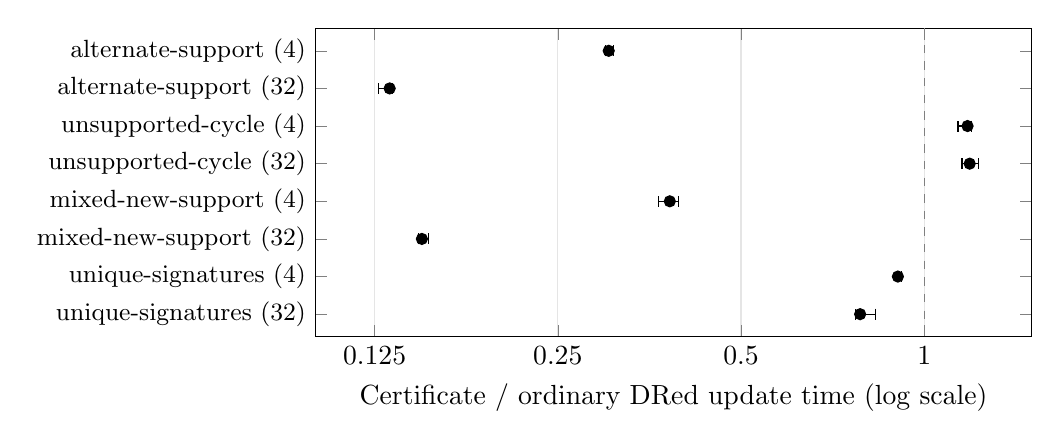
\begin{tikzpicture}
\begin{axis}[width=0.88\linewidth,height=5.5cm,xmode=log,
xmin=0.1,xmax=1.5,ymin=-0.6,ymax=7.6,
ytick={0,1,2,3,4,5,6,7},
yticklabels={alternate-support (4),alternate-support (32),unsupported-cycle (4),unsupported-cycle (32),mixed-new-support (4),mixed-new-support (32),unique-signatures (4),unique-signatures (32)},
yticklabel style={font=\small},y dir=reverse,
xlabel={Certificate / ordinary DRed update time (log scale)},
xtick={0.125,0.25,0.5,1},xticklabels={0.125,0.25,0.5,1},
xmajorgrids=true,grid style={gray!20}]
\addplot[gray,dashed] coordinates {(1,-0.6) (1,7.6)};
\addplot[only marks,mark=*,black,error bars/.cd,x dir=both,x explicit]
coordinates {
(0.303107186,0) += (0.005380192,0) -= (0.003875500,0)
(0.132315292,1) += (0.001499708,0) -= (0.005665689,0)
(1.178358201,2) += (0.016322907,0) -= (0.041958422,0)
(1.187932124,3) += (0.040023678,0) -= (0.034218154,0)
(0.381928514,4) += (0.012880738,0) -= (0.016163149,0)
(0.149473165,5) += (0.003692939,0) -= (0.001777688,0)
(0.905277511,6) += (0.011728574,0) -= (0.005298335,0)
(0.784898536,7) += (0.047034643,0) -= (0.012522867,0)
};
\end{axis}
\end{tikzpicture}
\caption{Post-hoc support replication. Points are median paired ratios; bars are descriptive paired-bootstrap intervals. Values left of one favor certificates; unsupported cycles expose their overhead.}
\label{fig:support}
\end{figure}


\subsection{Earlier production comparison with the fixed local baseline}
At commit \code{5531be4}, production kept union-first unary planning and ordinary
DRed; only the tested unary/binary lookup specialization was enabled from that
research phase. Its thesis suite contains 54 cases with five observations each. All 270
runs pass their checks; 51 cases match the preserved baseline's input hashes,
and three Bach additions are outside it. Table~\ref{tab:historical} reports
selected longitudinal comparisons, including costs. The full artifacts retain
all results, so this selection is not a summary of aggregate superiority.
\begin{table}[ht]
\caption{Selected historical medians (ms), five samples each. These are sequential local runs, not paired external-system comparisons. Materialization unless another operation is named.}
\label{tab:historical}
\centering\small
\begin{tabular}{@{}lrrr@{}}
\toprule
Workload/operation & b1254c4 & 8ce254f & 5531be4 \\
\midrule
Factored unions, width 64 & 10,406.030 & 119.371 & 105.388 \\
Enumerations, width 64 & 95.863 & 6.059 & 5.717 \\
Taxonomy D7/I15/PF & 4,860.310 & 4,388.391 & 4,777.663 \\
Same taxonomy: subsumption & 7,983.876 & 12.339 & 12.843 \\
Transitive, 100 & 451.250 & 710.512 & 446.153 \\
Cardinality D5/I3 & 243.571 & 367.386 & 227.536 \\
D5/10\% rule insert & 219.359 & 372.468 & 228.417 \\
D5/10\% rule replace & 417.815 & 725.576 & 457.058 \\
D5/10\% rule delete & 685.817 & 598.605 & 413.883 \\
D5/10\% atomic mixed & 771.007 & 709.321 & 791.637 \\
\bottomrule
\end{tabular}
\end{table}


Large cumulative gains on factored-union workloads and schema queries include earlier
modernization. They cannot be attributed to the experimental certificates or
adaptive selector, which are disabled. Sequential historical runs also differ
in environmental noise. The worst recorded materialization regression against
\code{b1254c4} is approximately 13.46\% on taxonomy D7/I9/P0. Neither this
single number nor an isolated large improvement substitutes for matched
competitive external evaluation.

\section{Established benchmarks and external evaluation}
\label{sec:external}
\subsection{Benchmark selection and comparison contracts}
The Lehigh University Benchmark (LUBM)~\cite{guo2005} is the first external workload because its maintainers supply
an ontology, deterministic generator, queries, and extensional reference
answers~\cite{lubmwebsite}. UOBM~\cite{ma2006} increases expressive and structural
demands; OWL2Bench~\cite{singh2020} provides explicit OWL 2 profile coverage.
ORE~\cite{parsia2017} supplies real-ontology reasoning tasks. WatDiv
\cite{aluc2014} and BSBM~\cite{bizer2009} instead stress RDF query processing.
Table~\ref{tab:benchmarks} identifies the relevant contracts rather than
treating these suites as interchangeable rankings.

For relational workloads, the Transaction Processing Performance Council's
Benchmark H (TPC-H) evaluates analytical queries over business
data~\cite{tpch}. Our use of selected query components is described below.

\begin{table}[ht]
\caption{Established benchmark candidates and their applicability. Selection is
our assessment; benchmark purpose and language come from the cited sources.}
\label{tab:benchmarks}
\small
\begin{tabularx}{\linewidth}{@{}p{.18\linewidth}YY@{}}
\toprule
Benchmark & Appropriate use & Required boundary \\
\midrule
LUBM & Loading, materialization, exact named query answers & Official ontology and generator; DLP L3 for the unmodified ontology here. \\
UOBM & More connected and expressive ontology workloads & Pin the generator: Oxford's version changes distributions; reject unsupported logical features. \\
Oxford maintenance suite & Compare DRed, DRed$^c$, B/F, B/F$^c$ & Match the exact transformed rule program and fact-deletion batches. \\
ORE 2015 & Coverage, consistency, classification, realization & Record unsupported ontologies; a filtered DLP track cannot inherit full DL/EL rankings. \\
OWL2Bench & Feature coverage and scaling by OWL 2 profile & Property chains and some other profile features exceed this compiler's contract. \\
WatDiv / BSBM & Join diversity and RDF query services & Separate query adaptation from inference; not tests of DRed or OWL completeness. \\
\bottomrule
\end{tabularx}
\end{table}

\subsection{Official LUBM(1,0): independent answer validation}
The initial external study uses UBA 1.7's unchanged bundled generator bytecode,
university index zero, seed zero, and one university. Fifteen department files
are generated. The original ontology IRI is retained; imports are resolved
locally and their 15 document import statements removed after resolution.
No logical ontology axiom is projected away. The resulting graph has 100,851
distinct triples, including 293 ontology triples. L2 rejects existential
consequents; DLP L3 accepts the original ontology and completes materialization.

The official query file contains punctuation errors and an older namespace.
The adapter records both the upstream bytes and its normalized queries, fixing
only those syntax/namespace differences. RDFLib parses each basic graph
pattern; the reasoner's existing indexed join evaluator executes it. This is
an explicit BGP adapter, not a complete SPARQL frontend. Bindings include named
individuals and literal values, matching the official extensional answers.
Skolem witnesses remain present in the materialization and in intermediate
reasoning.

All nine fresh workers (three configurations, three balanced blocks) return
exactly the official answer tuples for all fourteen queries: 126 successful
query checks, including both missing and excess tuple detection. In query
order, the cardinalities are
\begin{equation*}
(4,0,6,34,719,7790,67,7790,208,4,224,15,1,5916).
\end{equation*}
The full internal closure contains 234,480 facts; its named Univ-Bench projection
contains 138,478. All nine full internal closure hashes also agree. Internal
and named closure hashes are recorded separately; agreement does not independently certify every
unqueried existential consequence. Reference-answer equality is the stronger
external evidence for the named benchmark questions.

\begin{table}[ht]
\caption{Official LUBM(1,0), three fresh processes per configuration. Loading/reasoning times are seconds; the fully consumed fourteen-query total is milliseconds. Earlier current state is commit 5531be4.}
\label{tab:lubm}
\centering\small
\begin{tabular}{@{}lrrrr@{}}
\toprule
Configuration & Parse + reasoner & Compile & Materialize & Queries (ms) \\
\midrule
b1254c4 & 7.423 & 1.379 & 3.322 & 217.714 \\
current-fixed & 7.218 & 1.362 & 3.180 & 151.097 \\
current-adaptive & 7.387 & 1.395 & 3.310 & 150.822 \\
\bottomrule
\end{tabular}
\end{table}

Here ``current'' denotes the earlier \code{5531be4} research state, before the
subsequent optimizations motivated by the extended literature review. It is
preserved as a separate external control. The fixed variant has paired median
ratios of 0.957 for materialization and 0.6925 for the sum of fourteen query
times against \code{b1254c4}. This is a local same-host comparison, not a
comparison with the thesis's historical software. Three blocks and one
university establish neither robust scalability nor an external performance
frontier.

Query preparation is outside the query timer, and each query is fully consumed
once per worker. Cold denotes a fresh Python process, not a flushed operating
system filesystem cache. Compilation and materialization are subintervals of
reasoner construction; they must not be added to the already inclusive
parse-plus-reasoner column. Peak RSS includes RDF export and validation and is
approximately 984 MiB. The certificate mechanism concerns retractions and is
inactive in this static benchmark.

\subsection{Published reference results and what they establish}
The 2005 LUBM study~\cite{guo2005}, Table 1 (author PDF p.~15), reports
LUBM(1,0) loading times of 13 s for Sesame-Memory, 542 s for Sesame-DB, and
343 s for DLDB-OWL. Table 3 (author PDF p.~31) gives Q1 latencies of 15, 46,
and 59 ms respectively, all with four answers. Its 103,397-triple ABox count
includes duplicates. The machine was a 1.8 GHz Pentium 4 with 256 MB RAM,
Windows XP, Java 1.4.1, and a 512 MB heap; Sesame 1.0 used RDFS inference and
DLDB-OWL used its 2004-03-29 release. These loading, storage, and semantic
configurations differ from our DLP L3 materialization and BGP adapter. The numbers
are historical reference points and must not be divided by our times.

For the new maintenance hypothesis, the Oxford workloads are more relevant
than a query-only benchmark. Table~\ref{tab:published-maintenance} records two
verified rows from Hu et al.~\cite{hu2018}, Section 6 and Table 1 (author PDF
pp.~7--8). That study averages ten randomly selected 1,000-fact deletions on a
Dell PowerEdge R720 with two 2.6 GHz Xeon E5-2670 processors, 256 GB RAM, and
Fedora 24. It demonstrates why plain DRed alone is an insufficient competitive
control for a certificate optimization.

\begin{table}[ht]
\caption{Published small-deletion reference times from Hu et al.~\cite{hu2018}.
Seconds, on their hardware and transformed programs; these are not new runs.}
\label{tab:published-maintenance}
\centering\small
\begin{tabular}{@{}lrrrrr@{}}
\toprule
Program & Explicit facts & DRed & DRed$^c$ & B/F & B/F$^c$ \\
\midrule
Reactome-U & 12.5 million & 1.03 & 0.06 & 1.00 & 0.05 \\
UOBM-U & 254.8 million & 1,185.87 & 179.24 & 31.96 & 1.18 \\
\bottomrule
\end{tabular}
\end{table}

The U transformation is complete but unsound relative to the original OWL
ontology; R is sound but incomplete, and Claros-LE adds manually chosen rules.
These labels describe OWL approximation, not an error in Datalog evaluation of
the transformed program. The original counting artifact server could not be
retrieved during this study. No version-identical rerun of those Oxford data
or external DRed$^c$/B/F$^c$ executable is claimed.

Other widely used benchmarks expose different limitations. ORE evaluates
consistency, classification, and realization under DL/EL task limits; filtering
to supported DLP inputs changes the competition population. OWL2Bench includes
features such as property chains that this compiler currently rejects. WatDiv
uses diverse SPARQL patterns and BSBM includes service-level and aggregate query
workloads. Successful Horn closure does not implement those complete interfaces.
Their proper role is a separate coverage or query track, with unsupported
features and conversion costs recorded.

The final published RPT+ evaluation by Qiao, Boncz, and Zhang~\cite{qiao2026}
uses DuckDB 1.3.0 and eight threads on two Xeon Platinum 8474C processors with
512 GB DDR5 memory under Debian 12. Its benchmark population includes 18
TPC-H join queries at SF100, 113 Join Order Benchmark queries, eight Appian
queries, and 18,251 SQLStorm queries (13,308 completed, 2,837 failed, and 2,106
reached a ten-second timeout). Reported geometric-mean speedups are 1.17 for
TPC-H, 1.47 for JOB, 1.01 for Appian, and 1.28 for SQLStorm. The final PVLDB
paper is the reference here; an earlier author-hosted draft has different
numbers. Our smaller positive join components do not measure those full SQL
workloads, and their local speed ratios cannot be ranked against these values.

The pinned ZodiacEdge repository~\cite{zodiacartifact} reports LUBM(1) initial,
rule-insertion, and rule-deletion times of 588.9, 216.9, and 252.5 ms for the
$*$ subset, and 603.7, 56.3, and 21.5 ms for the $\#$ subset. These are author
README observations, separate from the paper's wind-turbine workloads with
aggregation and negation~\cite{xu2023}. Hardware, generation seed, repetition
count, and exact timing boundaries are not supplied for these README rows.
The supplied positive LUBM program nevertheless permits a stronger test: run
the author's unmodified engine and our implementation on one host with the
same facts, rules, update sequence, and validated semantic outputs.


\section{Follow-up implementation informed by the literature}
\label{sec:followup}
The literature review and the first experiment changed the optimization target.
The earlier selector saved inner-evaluator work while transaction preparation
dominated several complete updates. Changing-rule maintenance already has a
substantial history~\cite{volz2003maintenance,kotowski2011,xu2023}; recent join
research emphasizes the costs of execution choices and filtering
\cite{qiao2026}. We therefore implemented three further specializations and
evaluated them against both preserved commits and a same-source control.
These are engineering adaptations of established ideas. They neither implement
RPT+ nor replace B/F$^c$, modular maintenance, or a worst-case-optimal join.

\subsection{Reusing validation for monotone transactions}
The engine records the validated rule sequence, assertion set, and predicate
arities. An insertion-only transaction may reuse this certificate only when
the public rule and assertion containers still match it exactly. New facts and
rules are checked against the recorded arities and one another before the
transaction changes state. Submitted removals, a missing certificate, or direct
container mutation trigger complete validation. Deletion can release the last
occurrence fixing a predicate's arity, so applying the monotone shortcut there
would be unsound.

\begin{proposition}
For an unchanged validated input state whose embedded terms and identifiers
have stable values, equality, and hashes, checking the added facts and rules
against its arity map preserves the engine's input-validation conditions for
insertion-only transactions.
\end{proposition}
\begin{proof}
Groundness and permitted-term conditions on old facts, and rule safety and
permitted-term conditions on old rules, continue to hold because those objects
retain their structure and embedded values. These local conditions are checked on
every genuinely new object. The remaining shared condition is that every
occurrence of a predicate has the same arity. Extending a copy of the old arity
map while checking all new occurrences enforces that condition across old and
new objects and within the additions. The extended certificate is installed
only after these checks succeed.
\end{proof}

The API's frozen rule and atom records are shallow: arbitrary custom hashable
values can still have mutable internals. The stated stable-value assumption is
required for both the certificate and ordinary hash indexes. RDF terms and the
primitive identifiers used in these experiments satisfy it; snapshot equality
does not detect arbitrary in-place changes inside custom value objects.

When no rule is genuinely new, prepared plans are retained. A complete old
materialization has already registered its domain, including the private
nonempty-domain seed. Insertion of new rules therefore requires explicit
domain seeding only for their previously unseen constants; ingesting new facts
registers their own terms. Incomplete old states retain rematerialization.
Snapshot equality, assertion-set construction, and immutable snapshots still
incur work proportional to the existing state. This is a reduction in repeated
Python validation and preparation, not an $O(|\Delta|)$ bound for the complete
transaction.

\subsection{Maintaining surviving DRed indexes}
After overdeletion has finished using the old closure, ordinary DRed rebuilds
the index over the survivors. The candidate can instead erase each overdeleted
tuple from its relation and every corresponding column bucket. It uses erasure
when $2|D|\leq|I\setminus D|$, where $D$ is the overdeleted set and $I$ the old
indexed closure, and otherwise rebuilds. Empty buckets and relations are
removed. The threshold is an implementation heuristic, not a competitive
runtime guarantee.

For each relation $P$, column $j$, and value $v$, the index invariant is
\[
 B_{P,j,v}=\{t\in I_P:t_j=v\}.
\]
Erasing every $d\in D_P$ from $I_P$ and from $B_{P,j,d_j}$ leaves exactly the
buckets obtained by rebuilding over $I_P\setminus D_P$. Deletion occurs only
after the overdelete traversal, so its old-index access remains valid.
Rederivation then sees the same survivor index under either implementation.
The eligibility checks for equality, function terms, and complete old closures
are unchanged. This optimization reduces index construction costs; it does not
reduce the logical overdeletion set or solve incremental equality splitting.

\subsection{Positional bindings for ordinary positive joins}
For positive bodies without equality or inequality atoms, a reusable plan
assigns each variable a position in a binding vector. Atom terms are compiled
to variable positions or constant positions. Each recursive step retains the
existing dynamic choice of the smallest available exact index bucket, extends
a copied binding vector, and checks repeated variables. Constants are
canonicalized on every invocation because equality representatives can change.
The final vector is converted back to the original variable-binding interface.
Unary same-variable plans and the generic fallback remain available.

For validated bodies, the preservation argument is an induction on the remaining
body atoms; nonground Skolem patterns in bodies are rejected by validation. A
vector position represents exactly the binding of its corresponding variable.
The chosen index bucket is a superset of matches for the current partial
binding; constant and repeated-variable checks retain precisely the compatible
tuples. Every compatible extension recurses on the remaining atoms. At an
empty body, conversion preserves all bindings. Semi-naive evaluation keeps the
designated delta \emph{occurrence}, including when several atoms share a
predicate. Changing atom order does not change the set of substitutions.
This specializes an interpreter; it adds neither semijoin filtering nor the
Bloom-filter pipelines of Qiao et al.~\cite{qiao2026}.

Before the external timing series, the complete suite passed 698 tests. New
controls include 420 randomized insertion states, 140 randomized mixed
transactions with index comparisons, and 180 generated relational bodies
compared with an independent Cartesian-product evaluator. Tests also cover
failed-validation atomicity, public-container mutation, new domain constants,
equality fallback, and repeated delta predicates. These checks address the
implemented contracts rather than full OWL conformance.

\subsection{Matched author-program and SQL-component protocols}
The four local configurations are immutable commits \code{b1254c4} and
\code{5531be4}, the new source with all three switches disabled, and that same
source with all three enabled. The earlier adaptive unary selector and support
certificates remain disabled throughout. The same-source control distinguishes
the enabled bundle from changes that affect both paths. Comparing the bundle
does not isolate the contribution of each maintenance optimization.

The ZodiacEdge author repository~\cite{zodiacartifact} supplies a 128-rule
positive LUBM program and two marked rule subsets: eight rules marked $*$ and
sixteen marked $\#$, with one rule shared. Each scenario materializes without
the marked rules, inserts them, and removes them. Official UBA generation
provides 100,543 ABox facts after excluding ontology metadata. The author's
generation seed and file hashes are unavailable, so matching its published
input count is not proof of byte-identical data. The final author-program
closure has 238,474 non-domain tuples, including the 100,543 wrapped input
facts. It is a different semantic artifact from full-ontology DLP L3 reasoning.

Four balanced process blocks evaluate all four configurations. Ten fixed,
seeded samples each remove and reinsert 1,000 assertions under the complete
program. This follows the small-update scale used by Hu, Motik, and
Horrocks~\cite{hu2018}, but does not reproduce their Reactome or UOBM programs.
Thirteen fresh naive reference closures cover the full program, both partial
programs, and the ten fact-deletion states. Every timed worker checks complete
typed-tuple digests after every transaction outside the timer. The ten samples
within one worker are correlated: forty paired sample ratios are not forty
independent process replicates. Reported summaries are descriptive.

The Qiao-related component experiment uses official DuckDB \code{dbgen} data
at scale factors 0.01 and 0.1 and the positive joins underlying TPC-H Q3, Q5,
and Q9. It retains the original tables and filters, but projects every
participating row's complete primary key. Under the checked key constraints,
that projection identifies the entire tuple of input rows injectively and
therefore preserves the pre-aggregation SQL bag's multiplicity. Exact answers
are checked against independently executed SQL over the original database.
The engine's rule-free base closure is independently checked as its input
facts plus all required domain facts.

DuckDB performs date/string selections and projection; their time and complete
transfer to Python are recorded. Fact conversion, engine construction/indexing,
and complete join consumption are separate intervals, all included in the cold
component total. The three components run sequentially inside each fresh
worker, with a new reasoner per component but shared DuckDB and filesystem
caches. Aggregation, arithmetic, ordering, and top-$k$ are outside
this experiment. Three blocks, two scales, and four configurations yield 24
fresh workers and 72 component observations. Three rotations do not completely
balance four configurations. These small components are useful regression and
optimization probes, not a full TPC-H result or a reproduction of Qiao et al.'s
SF100 evaluation.

\subsection{Follow-up measurements}
\begin{table}[ht]
\caption{Author-supplied ZodiacEdge LUBM program: four fresh process blocks per configuration. Median seconds; initial includes engine construction and materialization. Parsing and outcome validation are outside these intervals.}
\label{tab:zodiac}
\centering\small
\begin{tabular}{@{}llrrr@{}}
\toprule
Subset & Configuration & Initial & Insert rules & Delete rules \\
\midrule
$\ast$ & b1254c4 & 3.5382 & 0.3338 & 2.3322 \\
$\ast$ & 5531be4 & 3.2811 & 0.3343 & 2.1418 \\
$\ast$ & current-fixed & 2.9002 & 0.3182 & 1.9661 \\
$\ast$ & candidate & 2.7809 & 0.1020 & 1.3576 \\
$\#$ & b1254c4 & 3.2615 & 0.4923 & 1.5962 \\
$\#$ & 5531be4 & 3.1646 & 0.4933 & 1.5541 \\
$\#$ & current-fixed & 2.7764 & 0.4403 & 1.4061 \\
$\#$ & candidate & 2.4551 & 0.2458 & 1.0838 \\
\bottomrule
\end{tabular}
\end{table}

\begin{table}[ht]
\caption{Supplemental 1,000-fact updates on the same author program. Median seconds across ten fixed subsets in each of four process blocks. These are forty correlated case/block observations per configuration.}
\label{tab:zodiac-facts}
\centering\small
\begin{tabular}{@{}lrr@{}}
\toprule
Configuration & Delete facts & Reinsert facts \\
\midrule
b1254c4 & 2.3727 & 0.1349 \\
5531be4 & 2.1627 & 0.1210 \\
current-fixed & 1.8719 & 0.1141 \\
candidate & 1.4258 & 0.0395 \\
\bottomrule
\end{tabular}
\end{table}

\begin{table}[ht]
\caption{Fully consumed join kernel for TPC-H-derived Q3/Q5/Q9 components (ms). Three fresh workers per scale/configuration. Final column is the median paired candidate/current-fixed ratio; smaller favors the candidate.}
\label{tab:tpch-joins}
\centering\small
\begin{tabular}{@{}llrrrrr@{}}
\toprule
SF & Join & b1254c4 & 5531be4 & Fixed & Candidate & Ratio \\
\midrule
0.01 & Q3 & 5.03 & 4.76 & 4.69 & 3.69 & 0.755 \\
0.01 & Q5 & 20.26 & 21.30 & 21.26 & 11.34 & 0.538 \\
0.01 & Q9 & 35.98 & 34.76 & 34.43 & 23.08 & 0.670 \\
0.1 & Q3 & 45.10 & 44.80 & 43.05 & 31.78 & 0.752 \\
0.1 & Q5 & 941.87 & 957.38 & 949.31 & 500.09 & 0.523 \\
0.1 & Q9 & 390.87 & 378.17 & 380.53 & 266.40 & 0.700 \\
\bottomrule
\end{tabular}
\end{table}

\begin{table}[ht]
\caption{Cold component total for TPC-H-derived Q3/Q5/Q9 components (ms). Three fresh workers per scale/configuration. Final column is the median paired candidate/current-fixed ratio; smaller favors the candidate.}
\label{tab:tpch-total}
\centering\small
\begin{tabular}{@{}llrrrrr@{}}
\toprule
SF & Join & b1254c4 & 5531be4 & Fixed & Candidate & Ratio \\
\midrule
0.01 & Q3 & 224.58 & 221.31 & 226.80 & 223.30 & 0.985 \\
0.01 & Q5 & 428.23 & 429.61 & 438.62 & 419.32 & 0.974 \\
0.01 & Q9 & 657.89 & 650.38 & 654.30 & 627.63 & 0.959 \\
0.1 & Q3 & 4,040.74 & 4,130.65 & 3,999.45 & 4,057.00 & 1.008 \\
0.1 & Q5 & 8,767.87 & 8,767.37 & 8,712.05 & 8,112.88 & 0.919 \\
0.1 & Q9 & 11,740.80 & 11,615.00 & 11,533.75 & 10,994.71 & 0.952 \\
\bottomrule
\end{tabular}
\end{table}


\subsection{An actual external engine on the same host}
The comparator uses the pinned, unmodified ZodiacEdge Program API and parser.
Its unary atoms use physical RDF type triples, whereas our store uses unary
relations. An injective encoding retains RDF term identity, and both outputs
are decoded to the same typed tuples for complete closure checks. Native input
index creation is included in initial compute. Conversion is recorded separately
and excluded from both implementations' compute intervals. Native whole-process
RSS includes adapter allocations, so it is not an isolated engine-memory ranking.
The program has no predicate variables; fixed predicate labels and injectively
encoded data constants occupy separate namespaces. Translating unary atoms to
type triples and binary atoms to property triples therefore gives a bijection
between rule substitutions. This validates the adapter's semantic contract;
full-run checks still test the engines' actual computation.
\begin{table}[ht]
\caption{Matched comparison with the unmodified author engine: four alternating paired blocks, seconds. Initial includes native input indexing. Final column is the median paired candidate/native ratio; below one favors our candidate.}
\label{tab:zodiac-native}
\centering\small
\begin{tabular}{@{}llrrr@{}}
\toprule
Subset & Operation & ZodiacEdge & Candidate & Ratio \\
\midrule
$\ast$ & Initial & 1.4001 & 2.4567 & 1.756 \\
$\ast$ & Insert rules & 0.5590 & 0.0880 & 0.161 \\
$\ast$ & Delete rules & 0.7850 & 1.1965 & 1.522 \\
$\#$ & Initial & 1.6595 & 2.1807 & 1.318 \\
$\#$ & Insert rules & 0.0589 & 0.2138 & 3.653 \\
$\#$ & Delete rules & 0.0234 & 0.9709 & 41.335 \\
\bottomrule
\end{tabular}
\end{table}


\subsection{Interpreting the maintenance improvement}
All 16 ZodiacEdge-program workers pass all 416 recorded complete-closure stage
checks. Relative to \code{b1254c4}, median paired insertion ratios are 0.3144
for $*$ and 0.4807 for $\#$, corresponding to 3.18-fold and 2.08-fold speedups.
Deletion ratios are 0.6119 and 0.6969. These are new matched local comparisons
on the author's program, not ratios against its published README times.

The same-source control is especially useful for attribution. Candidate/fixed
rule-insertion ratios are 0.3265 and 0.5470; deletion ratios are 0.7240 and
0.8230. Every individual paired update ratio favors the candidate in both
scenarios. For initial compute, however, the $*$ median ratio is 0.9770 and
two of the four individual ratios exceed one. We do not interpret that small
aggregate difference as a reliable initialization benefit. The $\#$ initial
ratio is 0.9051, with all four observations below one. No predeclared statistical
significance test or broad default-adoption criterion was attached to this
follow-up study.

Across the ten fixed 1,000-fact subsets and four blocks, pooled matched
candidate/\code{b1254c4} ratios are 0.6251 for deletion and 0.2808 for
reinsertion. Against the same-source fixed control they are 0.7169 and 0.3064.
These medians describe the sampled workload, with cases nested within processes.
They do not supply forty independent repetitions or establish the performance
of Oxford's larger UOBM or Reactome workloads.

The candidate preserves the original logical DRed work contract. For example,
in the first block it erases 24,933 indexed tuples for $*$ rule deletion and
24,045 for $\#$, rather than rebuilding all survivor buckets. Insertion can
reuse validated old inputs and plans. The experiment tests the combined changes;
it does not independently assign an exact portion of each speedup to validation,
index erasure, or positional joins. The original adaptive unary strategy and
proof certificates are disabled, so these results do not reverse their earlier
default-adoption findings.

\subsection{Positive-join gains and remaining intermediate work}
All 72 TPC-H component observations pass exact SQL row-identity and complete
base-closure checks. Paired candidate/fixed join ratios range from 0.523 to
0.755 over the six scale/component cases. The corresponding component totals
range from 0.919 to 1.008. Large Q5 improves about 47.7\% in the join interval,
but only 8.1\% in the sum of extraction, encoding, indexing, and joining.
Large Q3 does not show a component-total gain. These differences matter because
the Python loading and representation costs dominate this adapter.

Candidate and fixed configurations enumerate identical numbers of candidate
rows in every case. Q5 increases from 13,739 to 621,901 candidates between
SF0.01 and SF0.1, a 45.27-fold expansion for approximately tenfold input growth.
Positional bindings reduce interpretation cost but leave this join order
unchanged. This observation motivates the separately versioned lookahead
experiment below; it does not by itself identify the causal ordering decision.

The original component worker executes three queries sequentially. Later-query
fact encoding was faster in the candidate despite identical encoding logic.
Inspection found recursive local generator closures retaining captured state
until cyclic garbage collection. The earlier summed phase intervals exclude
explicit teardown and validation, so they are not all application CPU costs.
This is a plausible interaction, not a proven causal explanation of those
timings. The follow-up breaks the closure cycle in both new arms and gives each
component its own process, while retaining the original observations unchanged.

\subsection{The external comparison is mixed}
All eight native-comparison workers pass their six full-closure checks, giving
48 checked states. Relative to the unmodified ZodiacEdge engine, our candidate's
paired $*$ insertion ratio is 0.161, approximately a 6.2-fold improvement.
For $*$ deletion, however, the ratio is 1.522; for $\#$ insertion it is 3.653,
and for $\#$ deletion it is 41.335. Initial computation also favors ZodiacEdge.
One native $\#$ insertion is an outlier at approximately 0.215 seconds, compared
with approximately 0.058 seconds for the other three; all observations remain
in the artifact. Four paired blocks justify descriptive comparisons on these
operations, not a broad statistical or state-of-the-art ranking.

The large $\#$ deletion gap warrants diagnosis before another algorithmic claim.
Index erasure reduces physical rebuilding but leaves transaction-wide
preparation passes in place. A separately instrumented run, described below,
attributes most of this case's cost to those passes, while its overdeletion
set is exactly the set of lost facts. Thus this particular gap should not be
attributed to unnecessary logical overdeletion. Dependency-local maintenance
and safe reuse of validation evidence are relevant next directions, informed
by ZodiacEdge~\cite{xu2023} and modular materialization~\cite{hu2022modular}.

\subsection{Diagnostic profile of the rule-deletion gap}
\label{sec:deletion-diagnostic}
After the paired native comparison, we profiled one deletion of the sixteen
$\#$-marked rules using CPython 3.12.9 \code{cProfile}. The process used the
frozen primary candidate, its three enabled optimizations, the same 100,543
assertions and 128-rule program, and hash seed 7300. It first materialized the
partial program and inserted the marked rules; only their subsequent removal
was profiled. All three full typed-tuple closure checks passed. This is a
separate instrumented diagnostic, not an additional timing replicate.

The profiled public update accumulated 2.130745 seconds. Four disjoint call
groups accounted for 1.553658 seconds, or 72.9\%: canonicalizing all 100,543
assertions for protection, 0.551646 seconds; two checks of old and new DRed
eligibility, 0.520192 seconds; full input validation, 0.295590 seconds; and
recomputing active-domain constants, 0.186231 seconds. These cumulative times
include descendants but not one another. Nested normalization and literal-key
operations, or the enclosing DRed routine, must not be added again. All other
update work accounts for the remaining 0.577087 seconds. The engine's internal
update counter excludes validation and eligibility checks and therefore covers
a narrower interval.

Only sixteen rules were evaluated. The deletion overdeleted 24,045 facts and
rederived none, exactly matching the difference between the complete closures
of 238,474 and 214,429 tuples. Thus this observation contains no excess logical
overdeletion. Global preparation and protection passes dominate the observed
candidate cost. Since the native engine was not profiled, this result does not
quantitatively decompose the separately measured 41.3-fold runtime ratio or
show that eliminating those passes would close the gap.

Maintaining auxiliary state incrementally is established practice in view and
materialization maintenance~\cite{gupta1993,motik2019}; dependency analysis also
limits reconsideration under rule changes~\cite{kotowski2011,xu2023}. Applying
these general principles to the engine's metadata suggests eligibility
certificates, predicate occurrence counts, and active-domain reference counts.
The exact proposals here are not claims about the implementations in those
papers. Any certificate must detect relevant public-state changes and handle
datatype aliases and equality history. Arity counts must release a predicate's
constraint when its last occurrence disappears; domain counts must handle
constants supported only by removed rules and preserve the nonempty-domain
seed. Within an eligible DRed update, identity representatives also suggest
avoiding repeated canonicalization of unchanged assertions while preserving
inequality symmetry and domain protection.

These changes remain proposals, not implemented or measured improvements.
Deterministic profiling perturbs runtime, particularly for call-heavy Python
paths, and this single transaction cannot establish general workload behavior
or an achievable speedup. The compact artifact
\code{benchmarks/zodiac-deletion-profile.json} records frozen source and
profiler source hashes, the raw profile hash, independent closure checks,
nonoverlapping costs, and the instrumented engine counters.




\section{A post-hoc bounded join-order experiment}
\label{sec:lookahead}
The Q5 intermediate expansion prompted a second, separately frozen experiment.
The candidate draws on a lesson from RPT+ and Shredded Yannakakis
\cite{qiao2026,bekkers2025}: reducing intermediate work is useful only when
decision and reduction costs are included. It implements a smaller ordering
heuristic, with neither their filtering architecture nor their guarantees.

\subsection{Method and preservation argument}
At a recursive positive-join step, the candidate considers the two smallest
current index buckets only if the smaller contains at least 32 rows and the
larger is at most four times its size. For each candidate bucket it inspects
at most four physical rows, performs exact unification, and probes the other
remaining atoms. The score is the current bucket size multiplied by one plus
the average smallest next-step bucket size. A sampled row that fails repeated
variable or constant checks contributes zero next-step work. Ties retain the
original greedy choice. Samples are traversal estimates, never filters.

Hints are cached only for the invocation, keyed by remaining atom occurrences,
bound-variable positions, the two candidate occurrences, and bucket-size
bit-lengths. They contain an occurrence identifier, not answer bindings. This
coarse reuse may choose a poor order for a different binding, but cannot remove
an answer. The fixed limits are 1,024 additional index probes and 1,024 hints;
together they bound sampled physical rows by 8,192. A separate hint limit is
necessary because invalid sampled rows can consume no probes. Exhaustion uses
greedy evaluation, including ignoring already cached hints. These bounds do not
bound the cost of a poor chosen order or the query-width-dependent cost of
copying bindings and constructing keys.

\begin{proposition}
For a finite completed store and a validated positive relational query,
the bounded estimator preserves the complete substitution set of the
positional evaluator.
\end{proposition}
\begin{proof}
At each step the estimator chooses one remaining atom occurrence. The evaluator
then enumerates its entire selected index bucket and applies the same exact
compatibility tests as before. Every compatible extension recurses on precisely
the other occurrences. Induction on their number therefore yields all and only
the original substitutions. A misleading sample, reused hint, or exhausted
budget changes only the chosen occurrence. No estimate participates in a
compatibility test or in acceptance of a completed substitution.
\end{proof}

The implementation enables this path only for external headless queries on a
complete store. Installed rules, delta variants, incomplete stores, and
equality/difference builtins retain their existing evaluator. Hints are released
when the query ends. Independently of ordering, both new evaluator arms now
break a recursive local closure's self-reference on exhaustion, explicit close,
and exception. Tests with cyclic collection disabled check prompt release of
the captured engine and index. That lifecycle change is shared by the two new
arms, so their comparison isolates the ordering switch.

\subsection{Protocol}
Three balanced blocks compare \code{b1254c4}, the new compiled evaluator, and
that evaluator with lookahead. Each TPC-H component has its own fresh process;
two scales and three components therefore require 54 workers. Another 36
fresh workers evaluate near-unique, nonselective, skewed, and pairwise-consistent
but globally empty cyclic controls. The same hash seed is used within a block.
Sampling follows physical bucket order and is not a random statistical sample.

The unchanged original component definitions, SQL oracle, and row-identity
projection are reused. The new driver and package are archived separately;
the discovery study is not overwritten. Complete answer consumption, planning,
and recursive-closure cleanup are included in join time. The component total
adds extraction, encoding, and indexing. Complete process wall time additionally
includes startup, integrity hashing, validation, serialization, and teardown;
it is a reproducibility diagnostic rather than isolated query latency. Database
hashing warms filesystem caches, and the operating-system cache is not flushed.

This is a discovery-workload follow-up, not held-out validation. The parameter
values were fixed before its timed series; the preceding Q5 pilot is disclosed
and excluded from the timing summaries. Small independent finite-grounding
tests exercise constants, repeated variables/predicates, initial bindings,
budget exhaustion, and the zero-probe cache-bound case. Timed adverse controls
also compare with an independent nested-loop oracle. Lookahead remains
experimental and disabled by default.

\begin{table}[ht]
\caption{Single-component fresh-process study: median join milliseconds, followed by paired lookahead/compiled time ratios for join, component total, and complete process. Three balanced blocks; ratios below one favor lookahead.}
\label{tab:lookahead}
\centering\small
\begin{tabular}{@{}lrrrrrr@{}}
\toprule
Case & b1254c4 & Compiled & Lookahead & Join & Total & Process \\
\midrule
0.01/Q3 & 6.499 & 4.436 & 4.628 & 0.996 & 0.986 & 0.979 \\
0.01/Q5 & 58.258 & 48.740 & 49.326 & 1.001 & 1.016 & 1.011 \\
0.01/Q9 & 48.721 & 32.406 & 33.060 & 1.040 & 1.004 & 0.998 \\
0.1/Q3 & 58.692 & 42.424 & 43.047 & 1.015 & 1.001 & 1.003 \\
0.1/Q5 & 923.572 & 515.218 & 260.271 & 0.510 & 0.975 & 0.990 \\
0.1/Q9 & 398.469 & 262.076 & 272.030 & 1.043 & 1.000 & 0.998 \\
\bottomrule
\end{tabular}
\end{table}

\begin{table}[ht]
\caption{Synthetic adverse controls using the same protocol and columns as Table~\ref{tab:lookahead}. All planning and complete result enumeration are charged to the join interval.}
\label{tab:lookahead-controls}
\centering\small
\begin{tabular}{@{}lrrrrrr@{}}
\toprule
Case & b1254c4 & Compiled & Lookahead & Join & Total & Process \\
\midrule
unique & 0.316 & 0.283 & 0.309 & 1.123 & 1.019 & 0.990 \\
nonselective & 119.297 & 7.757 & 8.272 & 1.066 & 1.029 & 1.006 \\
skewed & 0.399 & 0.282 & 0.341 & 1.155 & 1.027 & 0.995 \\
empty-cycle & 0.296 & 0.177 & 0.220 & 1.238 & 1.064 & 1.008 \\
\bottomrule
\end{tabular}
\end{table}

\subsection{Results and adoption decision}
All 90 workers pass their independent answer and full base-closure checks.
At SF0.1, Q5 candidate visits fall from 621,901 to 155,969 in every block.
Each lookahead invocation performs 30 extra probes, examines 16 physical rows,
retains two hints, and changes 101 ordering choices. The paired
lookahead/compiled join ratio is 0.509923, with observed range
$[0.480504,0.519889]$. Against \code{b1254c4}, which also differs in earlier
indexing and interpreter improvements, the join ratio is 0.273615
$[0.268051,0.284502]$. These comparisons isolate ordering only when the
denominator is the same-source compiled arm.

The result does not establish a robust pipeline gain. Large-Q5 component-total
paired ratios are 0.975196 $[0.971553,1.272566]$, and process ratios are
0.990329 $[0.976037,1.284827]$. Separate component-total medians are 9.298 seconds
with lookahead and 7.307 seconds compiled, despite the median paired ratio
being below one. The block-specific shifts explain why the two summary
statistics differ; neither should be substituted for the other. One block has
a slower lookahead pipeline, largely in phases preceding query execution.
All observations are retained. The experiment did not control desktop activity
or processor affinity, and the preparation code is shared between these arms.
The data do not establish that lookahead caused the preceding-phase variation.

The other five TPC-H components keep their candidate-row counts unchanged.
Their paired join ratios range from 0.996 to 1.043, with the larger Q9 case
about 4.3\% slower. The four adverse-control join ratios are 1.123 for unique
joins, 1.066 for nonselective joins, 1.155 for skew, and 1.238 for the empty
cycle. Thus the extra decision machinery has measurable costs even when it
does not change the traversal. The very large nonselective improvement against
\code{b1254c4} is already present in the compiled control and must not be
attributed to lookahead.

The heuristic remains disabled by default. Its conditional Q5 success supports
further investigation of intermediate-sensitive ordering, while the adverse
results reject a universal benefit. No workload-specific dispatcher was tuned
on these final observations. The stored protocol was frozen locally before
measurement, not independently timestamped or publicly preregistered. This
post-hoc discovery-workload result establishes neither RPT+/SYA superiority
nor worst-case-optimal or no-regret evaluation.



\section{A matched existential task against a broader OWL reasoner}
\label{sec:hermit}
We compare immutable baseline \code{b1254c4}, the frozen follow-up candidate,
and HermiT~\cite{glimm2014hermit} on a finite DLP L3 entailment task. This is an
original controlled family, not an established corpus benchmark. It tests
computational specialization without assuming a frequency of suitable
ontologies in deployed applications.

\subsection{Input, task and independent semantic controls}
All arms receive identical RDF/XML bytes containing
\[
 A\sqsubseteq\exists R.B,\qquad \exists R.B\sqsubseteq C,
\]
with $N\in\{100,1000,10000\}$ named A instances, one further named B-only
individual, and an unrelated declared class D. Each worker establishes
consistency and retrieves all named C and D instances. The expected C answers
are exactly the $N$ A names; D has no entailed named instances.

The GCIs entail $A\sqsubseteq C$. A model with one shared B witness reached
from all A individuals, the B-only control outside C, and D empty satisfies
the ontology and establishes the negative-answer obligations. An empty
certain-answer set for D does not assert membership in its complement.
Removing either GCI permits a model with C empty. All nine separate preflight
processes---three arms on the full input and each omitted-GCI control---match
these independently justified answers. Ten small Python tests also pass,
including the semantic controls and rejection of a corrupted dependency jar.

Both existential axioms are essential to C entailment, but explicit witness
construction is not. HermiT uses its normal factory, classification and
realization behavior; the adapter does not replace the GCIs with
$A\sqsubseteq C$. We compare consistency and exact named answers, not complete
materializations or generated witness identities. The input family is also in
OWL 2 EL~\cite{owlprofiles2012}; a result against HermiT does not establish
superiority over specialized EL reasoners. Although the existential consequent
is outside structural RL, RDF-based subclass propagation can also answer this
particular C query.

\subsection{Pinned implementations and timing boundaries}
The candidate comes from the hash-verified
\path{benchmarks/followup-source.tar.gz}; it is the same package measured in
the ZodiacEdge and TPC-H follow-up studies, regardless of subsequent source
changes. The external distribution is the OWLAPI-maintained Maven artifact
\path{net.sourceforge.owlapi:org.semanticweb.hermit:1.4.5.519}, with OWLAPI
5.1.9. Its POM identifies it as a fork not officially supported by the original
HermiT developers.\footnote{Published artifact POM:
\url{https://repo.maven.apache.org/maven2/net/sourceforge/owlapi/org.semanticweb.hermit/1.4.5.519/org.semanticweb.hermit-1.4.5.519.pom}.}
The bundle and Maven metadata identify 1.4.5.519, while the API reports
1.4.1.513: bytecode inspection confirms that the pinned jar itself constructs
\code{Version(1,4,1,513)}. Both identifiers are retained. This comparison is
not a claim about the latest upstream distribution. Eleven downloaded Maven
artifacts and all 43 resulting classpath jars have recorded SHA-256 hashes.

Three blocks rotate the three arms by block and population position, giving
27 fresh processes on the same macOS 26.5.1 ARM64 host. Python is 3.12.9;
OpenJDK is 17.0.18 with \code{-Xms64m -Xmx2g}. The heap setting is not an
isolated memory measurement. All other timed studies were idle. A 180-second
worker limit, source/input hashes and order were recorded before measurement.
No worker failed, exceeded its limit or changed the measured source or input.
All 27 workers satisfy the exact answer and consistency contract.

Task time sums loading, reasoner construction, consistency, and fully consumed
C then D queries. Phase times are retained because eager DLP materialization
and lazy HermiT reasoning place work in different operations. A separate
parent timer covers the complete fresh process, including runtime startup,
answer serialization and exit. Input generation, dependency preparation,
Java compilation and the semantic preflight are excluded. The worker series
took 18.18 seconds. At $N=10000$, HermiT's median consistency and positive-query
phases take 1.176 and 0.903 seconds; a constructor-only comparison would omit
substantial work.

\begin{table}[ht]
\caption{Finite DLP L3 bridge task on identical RDF/XML inputs: median seconds over three fresh process blocks. Task includes loading, construction, consistency and both complete named-instance queries; process additionally includes runtime startup, answer serialization and exit.}
\label{tab:hermit}
\centering\small
\begin{tabular}{@{}rlrr@{}}
\toprule
Named A instances & Configuration & Task & Process \\
\midrule
100 & b1254c4 & 0.010029 & 0.101472 \\
100 & candidate & 0.009945 & 0.099147 \\
100 & HermiT & 0.220450 & 0.272145 \\
1,000 & b1254c4 & 0.086836 & 0.188231 \\
1,000 & candidate & 0.083865 & 0.178843 \\
1,000 & HermiT & 0.318659 & 0.372038 \\
10,000 & b1254c4 & 1.016922 & 1.135562 \\
10,000 & candidate & 0.937498 & 1.055745 \\
10,000 & HermiT & 2.475294 & 2.532972 \\
\bottomrule
\end{tabular}
\end{table}

\begin{table}[ht]
\caption{Within-block candidate/comparator ratios: median [minimum, maximum] over three pairs. Values below one favor the candidate. Ranges describe the measured pairs and are not confidence intervals.}
\label{tab:hermit-ratios}
\centering\small
\begin{tabular}{@{}rlll@{}}
\toprule
N & Comparator & Task ratio [range] & Process ratio [range] \\
\midrule
100 & b1254c4 & 0.985908 [0.978469, 1.077540] & 0.984859 [0.969318, 1.115056] \\
100 & HermiT & 0.046429 [0.044448, 0.049022] & 0.379001 [0.361144, 0.415761] \\
1,000 & b1254c4 & 0.965185 [0.957579, 0.990767] & 0.935610 [0.919415, 1.003251] \\
1,000 & HermiT & 0.262592 [0.259343, 0.263180] & 0.475576 [0.472795, 0.480711] \\
10,000 & b1254c4 & 0.950003 [0.716227, 0.994829] & 0.950974 [0.724435, 1.003096] \\
10,000 & HermiT & 0.378055 [0.372716, 0.400591] & 0.415056 [0.410029, 0.437214] \\
\bottomrule
\end{tabular}
\end{table}


\subsection{Observed computational value and its scope}
The candidate/HermiT paired median task ratios are 0.046429, 0.262592 and
0.378055 as $N$ increases; the corresponding full-process ratios are
0.379001, 0.475576 and 0.415056. Table~\ref{tab:hermit-ratios} reports the
complete observed ranges. HermiT loading dominates its smallest case, while
the advantage also persists in the complete process measurements. Relative
to \code{b1254c4}, the candidate's paired task ratios are 0.985908, 0.965185
and 0.950003. Most of its advantage over this HermiT artifact therefore
predates the new follow-up optimizations. Three blocks describe measured
variation; they do not establish a broad statistical population claim.
Within-block ratios need not equal ratios of marginal medians.

This demonstrates a useful implementation/task pairing with existential
axioms, independently of ontology prevalence. It does not prove a new
asymptotic bound, superiority over other EL or OWL implementations, or
termination/completeness on arbitrary recursive DLP L3 inputs. Raw phase timings,
exact-answer hashes, protocol and semantic controls are preserved in
\path{benchmarks/owl-bridge-results.json},
\path{benchmarks/owl-bridge-results-protocol.json} and
\path{benchmarks/owl-bridge-smoke.json}. The table generator checks worker
pairing, phase sums, answer hashes, protocol identity, marginal summaries and
every stored paired ratio before rendering these tables.


\section{Comparing the original Bach examples}
\label{sec:bach-comparison}

This comparison returns to the thesis's worked examples without enlarging them
or adding historical assertions. It distinguishes the complete ontology in
Table~2.5, p.~35, from the separate family maintenance example in Figure~6.2,
p.~150, Table~6.1, p.~151, and Example~6.3.2, pp.~158--159
\cite{volz2004}. The complete ontology uses the reconstruction's DLP L3 mode;
the family graph requires only its positive L0 rules. The examples' small
size makes them useful semantic tests, while limiting performance conclusions.

\subsection{Inputs, questions, and independent expectations}

The complete ontology retains T1--T17 and A1--A15. The displayed A16 is an
ellipsis and contributes no assertions. The supplied Turtle and RDF/XML
documents are checked for graph equivalence. The OWL comparisons use the same
RDF/XML bytes and 25 questions, covering named individuals, named relationships,
class descriptions, and schema properties. The current implementation and
the preserved \code{b1254c4} implementation are compared with the pinned
HermiT distribution described in Section~\ref{sec:hermit}. ZodiacEdge does not
provide the complete ontology's existence and constraint semantics through the
positive-rule interface evaluated here, so it has no full-ontology comparison.

The query expectations preserve the distinctions developed in the thesis.
Johann Ambrosius is a father because he is a man with a male child, although
that child is unnamed. The child is not thereby identified with Johann
Sebastian. Wilhelm Friedemann is recorded as a person; importing historical
knowledge to classify him as a man would change the answers to the
gender-qualified child questions. Marriage assertions alone do not imply
membership in the one-way definitions of \emph{Wife} or \emph{Husband}.
Empty named answers for birthday events do not deny the events required to
exist. Negative answers consistently mean absence of entailment, not entailed
negation. Generated witness identities and internal fact counts are not
cross-system answer criteria.

The reconstruction retains the documented scope decisions for Table~2.5 T12
and Example~5.4.2, pp.~133--134. The latter question explicitly applies its
person and gender conditions to the child. The father satisfiability question
does not imply that every possible fresh class assertion terminates under the
same procedure; the mutual existence requirements of \emph{Wife} and
\emph{Husband} remain outside such a conclusion.

The family input has nine asserted ancestor links and two initial rules:
ancestor transitivity and inclusion of ancestry in dynasty. Its nine questions
consist of the seven existing source-based questions and retrieval of both
complete named relations. The three changes independently replace one
ancestor assertion, remove the ancestor-to-dynasty rule, or add dynasty
symmetry. Each begins with the original input. Each incremental sequence also
reverses its change, providing a check that the original answers are restored.

Independent graph traversal establishes the expected relations. The original
state has 24 ancestor and 24 dynasty pairs. Replacing the Johann
Sebastian--Wilhelm Friedemann assertion by the Johann Sebastian--Johann
Christian assertion gives 25 pairs in each relation. Removing the inclusion
rule leaves 24 ancestor pairs and no dynasty pairs. Adding dynasty symmetry
leaves ancestry unchanged and produces 48 dynasty pairs. These are expected
logical counts, not internal storage counts. Every answer set is compared in
full, rather than accepted from its cardinality alone.

Two source corrections matter directly. The insertion notation on p.~159 is
resolved by its preceding prose and resulting deltas. Symmetry in the p.~151
example reverses ancestry pairs but does not connect the separate Johann
Christoph and Christoph branches. In particular, Johannes remains an ancestor
of Wilhelm Friedemann after the fact replacement because the path through
Maria Barbara survives. The thesis presents this retraction as a hypothetical
change to recorded knowledge, not a historical discovery about parentage.

Schema questions are not answered from accidental properties of the observed
relations. In the original state, dynasty happens to contain the same pairs
as ancestry, although its transitivity is not entailed. ZodiacEdge evaluates
these questions through fresh canonical assertions and the active positive
rules. The isolated rule evaluation tests the required implication; it does
not inspect the existing relation for apparent symmetry or transitivity.
Preparation and reasoning for these probes are charged to query time.

\subsection{Comparison matrix and timing boundaries}

The recorded design specifies twelve blocks of 28 fresh processes, giving
336 processes. Each block contains three complete-ontology runs, sixteen
family reconstructions, and nine incremental sequences. The reconstructions
cover four states in each of four systems. The sequences cover three changes
in the current implementation, the preserved baseline, and ZodiacEdge.
HermiT reconstructs the four family states; no incremental HermiT measurement
is claimed. System order rotates within blocks and benchmark processes run
sequentially. The protocol records the inputs, implementations, order, and
hash seeds before the timed series.

These are new observations of the preserved baseline implementation. Its
original saved benchmark report contained no Bach cases. The current source
is archived separately, and neither new measurement replaces earlier results.
Likewise, the earlier university rule-program comparison and the synthetic
existential HermiT comparison retain their original inputs and outcomes.

Static task time sums input and query preparation, conversion where required,
reasoner construction, consistency when supplied, and all fully consumed
answers. Phase times are retained because implementations defer different
amounts of work to queries. Query-specific reconstruction required by a local
API is included. Incremental task time includes preparation and application
of the change followed by the nine updated answers; original-state setup is
separate. The reverse change is also recorded and checked. ZodiacEdge's
mixed fact replacement uses its separate deletion and insertion calls, with
both included and no intervening query. This sequence is not described as an
atomic mixed update.

An independent outer measurement covers the full process, including runtime
startup, native bootstrap, checking, serialization, and shutdown. Source
preparation and Java compilation are outside the timed series. Process
restarts do not purge filesystem caches. The task intervals are reported as
defined phase sums, rather than assumed to account for every part of the
outer measurement. Absolute times are important on these small inputs, and
the comparison makes no claim about scaling to larger genealogies.

\subsection{Correctness outcomes and an external update discrepancy}

\begin{table}[ht]
\caption{Dissertation Bach examples, twelve repeated blocks. Median complete-task milliseconds, including all 25 full-ontology or nine family questions. Rebuilds include input preparation; updates exclude original-state setup. A failed configuration/task receives no timing ranking.}
\label{tab:bach-comparison}
\centering\small
\begin{tabular}{@{}lrrrr@{}}
\toprule
Task & Earlier baseline & Current & HermiT & ZodiacEdge \\
\midrule
Rebuild: Full ontology & 89.52 & 55.56 & 347.37 & -- \\
Rebuild: Original family & 9.41 & 7.49 & 269.67 & 4.43 \\
Rebuild: Fact replacement & 9.44 & 7.66 & 269.04 & 4.53 \\
Rebuild: Rule removal & 8.47 & 6.75 & 267.74 & 4.14 \\
Rebuild: Symmetry addition & 10.58 & 6.77 & 277.84 & 5.15 \\
Update: Fact replacement & 5.85 & 4.85 & -- & Failed (6/12) \\
Update: Rule removal & 4.77 & 4.00 & -- & 0.47 \\
Update: Symmetry addition & 6.53 & 3.64 & -- & 1.27 \\
\bottomrule
\end{tabular}
\end{table}

\begin{table}[ht]
\caption{Fresh-process wall time for the original Bach tasks, milliseconds. These intervals additionally include runtime startup, validation, serialization, and shutdown. Filesystem caches were not cleared.}
\label{tab:bach-process}
\centering\small
\begin{tabular}{@{}lrrrr@{}}
\toprule
Static task & Earlier baseline & Current & HermiT & ZodiacEdge \\
\midrule
Full ontology & 220.6 & 184.1 & 503.7 & -- \\
Original family & 136.6 & 135.6 & 416.3 & 137.9 \\
Fact replacement & 136.4 & 134.8 & 416.8 & 138.8 \\
Rule removal & 135.3 & 134.4 & 409.7 & 139.3 \\
Symmetry addition & 137.0 & 135.7 & 422.1 & 141.5 \\
\bottomrule
\end{tabular}
\end{table}


Separate diagnostic execution of the pinned ZodiacEdge version exposed a
loss of surviving support during fact replacement in some repeated executions.
The affected updated ancestor and dynasty relations omit the
Johannes--Wilhelm Friedemann pair despite the intact path through Maria
Barbara. The corresponding changed state has an independent graph-traversal
oracle and can also be evaluated from its assertions. This separates an
incremental-state discrepancy from ambiguity in the intended logical answer.
The observation is scoped to the tested version, input, and operation; it
does not establish the behaviour of other versions or all incremental methods.

The retained direct-API diagnostic in
\path{benchmarks/bach-native-deletion-diagnostic.json} reproduces the loss
without using the reconstructed reasoner, its ontology compiler, or the
comparison's schema-query probes. Native iteration can depend on object
identities as well as hash seeds, so selecting a seed does not guarantee the
same outcome in another process. The diagnostic and formal-run failure counts
describe the recorded executions; they are not estimates of a general failure
probability.

Failed executions, their diagnostics, and any answers emitted before failure
remain in the raw record. Any failed execution disqualifies its complete
system--task combination from timing rankings, rather than leaving a median
computed from selected successful executions. Unsupported comparisons are
reported separately from wrong answers or failures to complete. The earlier
successful checks on ZodiacEdge's university rule changes remain evidence
about those particular tasks, not a guarantee that every other change is
handled correctly.

Raw observations and the frozen protocol are retained in
\path{benchmarks/bach-external-results.json} and
\path{benchmarks/bach-external-results-protocol.json}.
The candidate source and actual generated inputs are preserved separately in
\path{benchmarks/bach-external-source.tar.gz} and
\path{benchmarks/bach-external-inputs.tar.gz}.
The paper preparation step checks the answer contracts, pairing, and timing
eligibility before producing the result table and records the evidence files'
digests. Rebuilding the manuscript does not rerun the experiments.


\section{Final default configuration and baseline validation}
The production configuration now enables monotone validation/plan reuse,
incremental survivor-index maintenance, and positional positive joins. It also
includes the recursive-closure lifecycle correction. Adaptive unary planning,
shared support certificates, and the new lookahead remain disabled. The final
package is preserved in the later lookahead source archive; it differs from
the primary follow-up archive, whose switches were enabled at runtime and which
predates the lifecycle correction.

The complete source passes 741 tests, lint, both independent thesis
counterexample scripts, the original research-artifact validator, and a source
and wheel build. The final thesis suite contains 54 fresh case workers, each
with five observations: all 270 observations pass the workload's checks. All
51 historical cases match the fixed \code{b1254c4} input hashes and correctness
controls. The three Bach cases also pass but lie outside that baseline's
coverage. Recorded package hashes match the frozen later archive; source
integrity is checked throughout the suite.

\begin{table}[ht]
\caption{Final default configuration, selected historical medians in milliseconds (materialization unless specified). Five observations per case, sharing one worker. The ratio is final/b1254c4; these longitudinal observations are not an interleaved comparison.}
\label{tab:final-production}
\centering\small
\begin{tabular}{@{}lrrrr@{}}
\toprule
Workload/operation & b1254c4 & 5531be4 & Final & Ratio \\
\midrule
Unions, 64 pairs & 10,406.030 & 105.388 & 82.267 & 0.008 \\
Enumerations, 64 pairs & 95.863 & 5.717 & 4.358 & 0.045 \\
Taxonomy D7/I15/PF & 4,860.310 & 4,777.663 & 3,336.927 & 0.687 \\
Same: subsumption & 7,983.876 & 12.843 & 9.338 & 0.001 \\
Transitive, 100 & 451.250 & 446.153 & 317.792 & 0.704 \\
Cardinality D5/I3 & 243.571 & 227.536 & 166.633 & 0.684 \\
D5/10\% rule insert & 219.359 & 228.417 & 225.281 & 1.027 \\
D5/10\% rule replace & 417.815 & 457.058 & 200.632 & 0.480 \\
D5/10\% rule delete & 685.817 & 413.883 & 181.603 & 0.265 \\
D5/10\% atomic mixed & 771.007 & 791.637 & 284.407 & 0.369 \\
D4/15\% fact insert & 24.074 & 24.232 & 30.287 & 1.258 \\
\bottomrule
\end{tabular}
\end{table}

All 51 recorded materialization medians are lower than the saved baseline in
this run, with ratios ranging from 0.00791 to 0.83264. The very large factored
expression and schema-query differences include the preceding modernization;
they cannot be assigned to the latest three changes. These observations also
include naive and OWL-RL controls, and historical runs were neither interleaved
nor isolated from host drift. The result is a longitudinal regression check,
not a causal effect estimate or external-system ranking.

Maintenance is not uniformly faster. Of the 36 case/operation comparisons,
34 have lower update medians, while D4/15\% fact insertion is 25.8\% slower
and D5/10\% rule insertion is 2.7\% slower than the saved baseline. These costs
are retained in the table and raw data. The matched external experiments give
more focused attribution evidence than these sequential historical comparisons.
The final observations are stored separately in
\path{benchmarks/followup-thesis-results.json}; neither the original baseline
nor the preceding production results are overwritten.


\section{Are DLP fragments still worthwhile alongside OWL 2 RL?}
\label{sec:profiles}
Our answer separates theoretical and computational merit from practical
adoption. A fragment can be worthwhile even when its prevalence in deployed
ontologies is unknown. DLP remains useful as a foundation and as a decomposition
of evaluator capabilities. OWL 2 RL explicitly credits DLP among its
influences~\cite{owlprofiles2012}; standardization incorporated the central
idea rather than making it irrelevant.

In particular, DLP L3's existential consequents can express useful statements
beyond RL's syntax. If specialized DLP L3 reasoning is faster than a more expressive
OWL reasoner on the same DLP L3 inputs and reasoning tasks, while preserving the
same correctness and completeness obligations, that is evidence for a useful
computational fragment. No estimate of how often users need only DLP L3 is required
for this conclusion. The finite existential-bridge study in
Section~\ref{sec:hermit} now supplies such scoped computational evidence:
the preserved baseline and candidate both answer the same consistency and
named-instance task faster than the pinned broader-language HermiT
distribution~\cite{glimm2014hermit}. All 27 measured workers match independently
justified answers. The candidate/HermiT paired median task ratios are
0.046429, 0.262592, and 0.378055 for 100, 1,000, and 10,000 named A instances;
the corresponding full-process ratios are 0.379001, 0.475576, and 0.415056.
These are results for one controlled family and three process blocks, not a
new complexity bound or a comparison with every broader-language OWL implementation.
Most of this advantage is already present in the fixed baseline.

Measured advantages and mathematical guarantees provide different evidence.
One can prove an expressiveness--complexity tradeoff without an adoption survey;
one can also demonstrate an implementation advantage without proving a new
complexity separation. Hustadt, Motik, and Sattler~\cite{hustadt2005} establish
P-complete data complexity for basic Horn-SHIQ reasoning, while general SHIQ
instance checking is coNP-complete under their assumptions. This is an example
of prior theoretical justification for expressive Horn fragments. It does not
identify our DLP L3 with Horn-SHIQ or give our unrestricted witness chase that bound.
Termination, combined complexity, data complexity, and query complexity require
their own precise language and task definitions.
In particular, nontermination of this Skolem chase is a limitation of the
chosen procedure, not by itself a proof that reasoning in the original
description-logic fragment is undecidable.

Three classifications must remain distinct: the thesis's constructor-position
fragments, the actual RDF encodings accepted by this compiler, and the
conditions under which an optimization is valid. An L0 ontology can contain
expensive transitive binary joins. An ontology accepted with the L2 ceiling may
contain only unary implications. Choosing a higher ceiling does not add absent
equality or constraints, and a label alone cannot predict cost.

\subsection{Overlap rather than automatic profile inclusion}
Concrete syntax witnesses rule out identifying these labels with RL subsets.
The DLP L3 inclusion $A\sqsubseteq\exists R.B$ has a general existential
consequent absent from RL's superclass grammar. Even L1's $\top\sqsubseteq A$
is outside its subclass grammar. Conversely, RL supports restricted property
chains and keys, which this compiler rejects~\cite{owlprofiles2012}. These
are statements about syntactic membership, not impossibility of equivalent
rewriting or a claim that DLP L3 contains RL.

Global restrictions matter independently. The compiler accepts simultaneous
transitivity and functionality of the same property. That rule set has a
first-order interpretation, but the property fails OWL 2 DL's simplicity
condition for functionality~\cite{owlsyntax2012}. Parser acceptance therefore
does not certify a standard OWL 2 RL ontology. Datatype completeness is another
separate gap in this implementation.

OWL 2 RL/RDF rules can also be applied beyond syntactically conforming RL.
Their Direct-Semantics correspondence has explicit conditions, including
restrictions on entity roles and on the conclusions covered by the theorem
\cite{owlprofiles2012,owlconformance2012}. A comparison must choose its
semantic contract. Our equality acts on individual arguments, not predicate
identifiers. Requiring identity with every triple produced by an RDF-Based
reasoner can therefore demand consequences outside the intended contract.

\subsection{What restrictions can still buy}
For this implementation, function freedom gives finite active-domain
materialization. Eligible states without explicit or datatype-induced equality
avoid representative splitting during
deletion. Same-variable unary bodies permit set-intersection evaluation.
These properties are useful internal dispatch conditions, including within a
broader supported ontology. They do not require presenting another public
ontology language as a replacement for RL.

A small compiler can also be easier to audit and reproduce. Its value depends
on real schemas fitting the contract and on explicit rejection of unsupported
axioms. Conversion costs, excluded standard features, and additional
conformance work are part of the cost of the restriction. The earlier
certificate and unary experiments demonstrate workload-specific benefits and
failures, not an advantage of requiring a DLP frontend over accepting the same
axioms through a conforming RL frontend.

LUBM illustrates the distinction between ontology coverage and query
sufficiency. Its full ontology needs this implementation's DLP L3 mode, and all
fourteen named answer sets match. That does not prove those questions require
generated witnesses. Nor would matching them after a projection prove ontology
equivalence. Existential consequences can affect named answers: from $A(a)$,
$A\sqsubseteq\exists R.B$, and $\exists R.B\sqsubseteq C$, we obtain $C(a)$
\cite{owldirect2012}. Dropping the witness-producing inclusion without a
justified rewriting loses this consequence.
The HermiT study evaluates precisely this bridge together with a B-only
negative individual and an unrelated empty-answer class. Both GCIs are
essential to the answer, but explicit witness construction is not: the TBox
entails $A\sqsubseteq C$, and HermiT retains its normal optimizations. The
family also belongs to OWL 2 EL, so the result does not establish superiority
over specialized EL reasoners. It compares the specified entailment task,
not entire materializations or generated witness identities.

\subsection{Practical adoption is a separate question}
OWL 2 EL and QL supply other established tradeoffs, respectively oriented toward
large terminologies with existential descriptions and query rewriting over
large instance data~\cite{owlprimer2012}. They are alternatives to evaluate,
not automatic solutions for every DLP L3 query. In particular, avoiding explicit
infinite witness expansion for classification does not establish completeness
for arbitrary conjunctive queries or cardinality constraints.

The frequency with which real applications need only DLP L3 is a difficult empirical
question. Published ontology collections can reveal supported constructs in
those collections, but may be unrepresentative; they also do not fully reveal
application queries, update needs, or equivalent rewritings. We do not require
an answer to that question before recognizing a fragment's theoretical value.

For practical interoperability claims, checked standard profiles and explicit
extensions would complement the historical DLP L0--L3 interface. A deployment study
could measure coverage and rejection reasons, full input-to-answer and update
costs, conversion and memory, and ablations with compiled rules held fixed.
Its coverage conclusions would remain specific to the sampled population.
Current evidence supports the fragments as foundations and research targets
and demonstrates a computational advantage on the stated existential task.
That scoped result stands independently of prevalence; it does not establish
the historical interface as a better interoperability standard or settle
performance on other ontology and query families.


\appendix
\section{Reproducibility and provenance}
\label{app:repro}
The original thesis file has SHA-256
\begin{quote}\small\ttfamily
80146ec324e0a7c342508e38cbe7712f207db8917d6655cd70b9acbcaee2f570
\end{quote}
and the pinned \code{b1254c4} result file has SHA-256
\begin{quote}\small\ttfamily
6f0bc493cae0fb96b474405eb9496dc9ce2c3155b313f2bcd3de49b3dc8b51e2.
\end{quote}
The source archive, protocols, raw primary observations, post-hoc replication,
and final production observations are distinct files. Their measurement
boundaries must remain distinct when recomputing summaries. Tables of our new
benchmark measurements are generated from these JSON artifacts. Published
reference values are separately attributed to their sources. The preparation
script records input digests.

The principal existing checks and reproduction commands are:
\begin{verbatim}
uv sync --extra dev --locked
uv run pytest -q
uv run ruff check src tests benchmarks scripts
uv run python scripts/check_thesis_logic.py
uv run python scripts/check_thesis_errata.py
uv run python scripts/validate_research_artifacts.py
uv run python scripts/replay_support_research.py \
  --output /tmp/dlp-support-reproduction.json
uv run python -m benchmarks.run --suite thesis --repeats 5 \
  --output /tmp/dlp-thesis-reproduction.json
\end{verbatim}
Heavy timed reproductions should run sequentially. They record their own source
and runtime state and are not replacements for the archived observations.
The raw primary worker assertion/rule digests describe the expected candidate;
the integration tests independently check the actual internal candidate state.
The post-hoc replication checks original-report, driver, protocol, and source
hashes and uses seeds 3000--3008.

The manuscript uses George Kour's MIT-licensed \code{arxiv-style} template,
pinned by commit and file digest in \code{template-provenance.json}. This is a
community preprint style, not an official arXiv endorsement. The source package
includes the local style and compiled bibliography, uses standard pdfLaTeX
packages, requires no shell escape, and can be rebuilt without benchmark
execution or network access. The repository's paper README documents the
build, external dataset preparation, and packaging commands.

\setlength{\bibsep}{1pt}
\renewcommand{\bibfont}{\small\raggedright}
\bibliographystyle{plainnat}
\bibliography{references}
\end{document}
